\SourcePage{86}
\SGAsection{5}{Weyl 群：生成元与关系}
设 $\mathscr R$ 是一个\Term{root-datum}{根数据}。由于它的\Term{weyl-group}{Weyl 群}与相应\Term{reduced-root-datum}{约化根数据}的\Term{weyl-group}{Weyl 群}相同，研究\Term{weyl-group}{Weyl 群}时可以假设 $\mathscr R$ \Term{reduced}{约化}。
设 $\Delta=\{\alpha_1,\ldots,\alpha_n\}$ 是一个\Term{simple-root-system}{单根系}（$n=\operatorname{rgss}(\mathscr R)$）。记 $n_{ij}$ 为 $W$ 中元素 $s_{\alpha_i}s_{\alpha_j}$ 的阶。特别地，$n_{ii}=1$；在 3.4.2 和 3.4.3 中已经看到，由 $s_{\alpha_i}$ 与 $s_{\alpha_j}$ 生成的 $W$ 的\Term{subgroup}{子群} $W_{ij}$ 由关系
\[s_{\alpha_i}^2=s_{\alpha_j}^2=(s_{\alpha_i}s_{\alpha_j})^{n_{ij}}=1\]
定义。
\begin{SGAresult}{定理}{5.1}
群 $W$ 是由元素 $s_{\alpha_i}$（$i=1,2,\ldots,n$）生成、满足关系 $(s_{\alpha_i}s_{\alpha_j})^{n_{ij}}=1$ 的群。
\end{SGAresult}
\begin{proof}
已经知道 $n=2$ 时定理成立；证明中将用到这一点。引入由元素 $T_i$（$i=1,2,\ldots,n$）生成、满足关系 $(T_iT_j)^{n_{ij}}=1$ 的群 $\overline W$。特别地，由 $n_{ii}=1$ 得 $T_i^2=1$。设 $p:\overline W\to W$ 是将 $T_i$ 送至 $s_{\alpha_i}$ 的群\Term{morphism}{态射}。已知 $p$ \Term{surjectivity}{满射}，下面证明它\Term{injectivity}{单射}。
\begin{SGAresult}{引理}{5.2}
可以唯一地对每个 $\alpha\in P(\Delta)$ 定义元素 $T_\alpha\in\overline W$，使它们具有以下性质：
\begin{enumerate}
\item[(i)] $p(T_\alpha)=s_\alpha$；
\item[(ii)] $T_{\alpha_i}=T_i$；
\item[(iii)] 若 $\beta$ 和 $\alpha$ 是两个\Term{positive-root}{正根}且 $s_{\alpha_i}(\alpha)=\beta$，则 $T_iT_\alpha T_i=T_\beta$。
\end{enumerate}
\end{SGAresult}
\SourcePage{87}
首先，由 1.2.10 与 3.3.6 可知，(i) 是 (ii) 和 (iii) 的推论，而 (ii) 和 (iii) 完全确定 $T_\alpha$。下面对 $\operatorname{ord}_\Delta(\alpha)$ 归纳构造。当 $\operatorname{ord}_\Delta(\alpha)=1$ 时，$\alpha\in\Delta$，若 $\alpha=\alpha_i$，就置 $T_\alpha=T_i$。考虑假设：
\begin{quote}
$(H_p)$ 对 $\alpha\in P(\Delta)$、$\operatorname{ord}_\Delta(\alpha)\leq p$，存在满足 (ii) 的 $T_\alpha$，并在 $\operatorname{ord}_\Delta(\alpha)\leq p$、$\operatorname{ord}_\Delta(\beta)\leq p$ 时满足条件 (iii)。
\end{quote}
$p=1$ 时此假设成立：事实上，若 $\alpha$ 与 $s_{\alpha_i}(\alpha)=\beta$ 都是\Term{simple-root}{单根}，则 $\alpha_i$ 与 $\alpha$ \Term{orthogonality}{正交}；因此若记 $\alpha_j=\alpha=\beta$，则 $n_{ij}=2$，从而
\[T_iT_jT_i=T_j.\]
现设 $p>1$ 且 $(H_{p-1})$ 成立。

A）构造 $\operatorname{ord}_\Delta(\alpha)\leq p$ 时的 $T_\alpha$。显然只需对 $\operatorname{ord}_\Delta(\alpha)=p$ 构造。此时存在 $\alpha_i\in\Delta$，使 $s_{\alpha_i}(\alpha)\in P(\Delta)$ 且 $\operatorname{ord}_\Delta(s_{\alpha_i}(\alpha))<p$（3.3.3）。于是置
\[T_\alpha=T_iT_{s_{\alpha_i}(\alpha)}T_i.\tag{$\star$}\]
验证 $T_\alpha$ 只依赖于 $\alpha$。设 $\alpha_j\in\Delta$ 也满足 $s_{\alpha_j}(\alpha)\in P(\Delta)$ 且 $\operatorname{ord}_\Delta(s_{\alpha_j}(\alpha))<p$。要证明
\[T_iT_{s_{\alpha_i}(\alpha)}T_i=T_jT_{s_{\alpha_j}(\alpha)}T_j.\tag{+}\]
分为两种情形。

（1）设 $\alpha$ 是 $\alpha_i$ 和 $\alpha_j$ 的线性组合。于是 $s_{\alpha_i}(\alpha)$ 和 $s_{\alpha_j}(\alpha)$ 也是如此；由 $(H_{p-1})$，$T_{s_{\alpha_i}(\alpha)}$ 与 $T_{s_{\alpha_j}(\alpha)}$ 都能写成 $T_i$、$T_j$ 构成的字。由于 $(+)$ \Term{projection}{投影}到 $W$ 后成立，而定理对 $n=2$ 成立，即 $p$ 在 $\overline W$ 中由 $T_i,T_j$ 生成的\Term{subgroup}{子群}上\Term{injectivity}{单射}，故 $(+)$ 成立。

（2）设 $\alpha$ 不是 $\alpha_i$ 和 $\alpha_j$ 的线性组合。于是，对 $w\in W_{\alpha_i\alpha_j}$，各 $w(\alpha)$ 都是\Term{positive-root}{正根}（参见 3.4.9）。待证关系也可写成
\[(T_iT_j)^{n_{ij}-1}T_{s_{\alpha_i}(\alpha)}(T_jT_i)^{n_{ij}-1}=T_{s_{\alpha_j}(\alpha)}.\tag{++}\]
由 4.4，当 $w\in W_{\alpha_i\alpha_j}$、$w\ne1$ 时，所有 $w(\alpha)$ 的\Term{root-order}{阶}均小于 $p$。因而\Term{continuous}{连续}应用 $2(n_{ij}-1)$ 次假设 $(H_{p-1})$ 即可。

B）验证 $(H_p)$。\footnote{编者注：下面补充了原文的细节。}须验证：若 $\alpha_j\in\Delta$，且 $\beta=s_{\alpha_j}(\alpha)$ 满足 $\operatorname{ord}_\Delta(\beta)\leq p$，则 $T_jT_\alpha T_j=T_\beta$。若 $\operatorname{ord}_\Delta(\beta)<p$，由上面的论证（以及 $T_j^2=1$）即可得出；故可设 $\operatorname{ord}_\Delta(\beta)=p=\operatorname{ord}_\Delta(\alpha)$。此时 $\alpha$ 与 $\alpha_j$ \Term{orthogonality}{正交}，故 $\beta=\alpha$，需要证明的是
\[T_jT_\alpha T_j=T_\alpha.\tag{$\dagger$}\]
\SourcePage{88}
由上面的 $(\star)$，$T_\alpha=T_iT_{s_{\alpha_i}(\alpha)}T_i$，所以只剩下验证等式
\[T_jT_iT_{s_{\alpha_i}(\alpha)}T_iT_j=T_\alpha=T_iT_{s_{\alpha_i}(\alpha)}T_i.\tag{+++}\]
记 $m=n_{ij}$，$s_i=s_{\alpha_i}$、$s_j=s_{\alpha_j}$。有 $T_jT_i=(T_iT_j)^{m-1}$，而由 4.4，对 $W_{ij}$ 中不同于 $1=(s_is_j)^m$ 和 $s_j=s_i(s_is_j)^{m-1}$ 的所有 $w$，均有 $\operatorname{ord}_\Delta(w(\alpha))<p$。于是由归纳假设得
\[T_j(T_iT_j)^{m-2}T_{s_i(\alpha)}(T_jT_i)^{m-2}T_j
=T_{s_j(s_is_j)^{m-2}s_i(\alpha)}=T_{s_is_j(\alpha)}=T_{s_i(\alpha)}\]
（最后的等式是因为 $s_j(\alpha)=\alpha$），从而最终有
\[(T_iT_j)^{m-1}T_{s_i(\alpha)}(T_jT_i)^{m-1}=T_iT_{s_i(\alpha)}T_i,\]
这就证明了 $(+++)$，也证明了引理。
\begin{SGAresult}{引理}{5.3}
设 $h\in\overline W$，将它写成
\[h=T_{\alpha_1}\cdots T_{\alpha_m},\]
其中 $\alpha_i\in\Delta$，不必互异，并使 $m$ 最小。则
\[p(h)(\alpha_m)\in-P(\Delta).\]
\end{SGAresult}
事实上，由于 $p(T_{\alpha_m})(\alpha_m)=s_{\alpha_m}(\alpha_m)=-\alpha_m$，若 $p(h)(\alpha_m)$ 为\Term{positive-root}{正根}，就存在指标 $k$，$1\leq k\leq m-1$，使
\[u=s_{\alpha_{k+1}}\cdots s_{\alpha_m}(\alpha_m)
=-s_{\alpha_{k+1}}\cdots s_{\alpha_{m-1}}(\alpha_m)\in-P(\Delta),\]
且 $s_{\alpha_k}(u)\in P(\Delta)$。但此时必有 $u=-\alpha_k$（3.3.1），故
\[s_{\alpha_{k+1}}\cdots s_{\alpha_{m-1}}(\alpha_m)=\alpha_k,\]
由 (iii) 可得
\[T_{\alpha_k}T_{\alpha_{k+1}}\cdots T_{\alpha_{m-1}}T_{\alpha_m}
=T_{\alpha_{k+1}}\cdots T_{\alpha_{m-1}},\]
这与 $m$ 的最小性矛盾。

现设 $h\in\overline W$ 满足 $p(h)(P(\Delta))\subset P(\Delta)$。由引理 5.3，有 $p(h)=1$；这就证明了定理 5.1，并且还得到下述推论。
\end{proof}
\begin{SGAresult}{推论}{5.4}
若 $R_+$ 是一个\Term{positive-root-system}{正根系}，且 $w\in W$ 满足 $w(R_+)=R_+$，则 $w=1$。
\end{SGAresult}
\begin{SGAresult}{推论}{5.5}
\Term{weyl-group}{Weyl 群}在\Term{positive-root-system}{正根系}的\Term{set}{集合}上（分别在\Term{simple-root-system}{单根系}的\Term{set}{集合}上、\Term{weyl-chamber}{Weyl 室}的\Term{set}{集合}上）自由且传递地\Term{action}{作用}。
\end{SGAresult}
现在选定一个\Term{simple-root-system}{单根系} $\Delta$，置 $R^+=P(\Delta)$。\footnote{编者注：这里将 $R_+$ 写成 $R^+$，以便记 $R_{\alpha,\beta}^+=R_{\alpha,\beta}\cap R^+$。}对每一对\Term{simple-root}{单根} $(\alpha,\beta)\in\Delta\times\Delta$，记 $R_{\alpha,\beta}$ 为所有能写成 $\alpha,\beta$ 的线性组合的\Term{root}{根}的\Term{set}{集合}。记 $R_{\alpha,\beta}^+=R^+\cap R_{\alpha,\beta}$，并设 $W_{\alpha,\beta}$ 是 $R_{\alpha,\beta}$ 的\Term{weyl-group}{Weyl 群}，即 $W$ 中由 $s_\alpha,s_\beta$ 生成的\Term{subgroup}{子群}。
\SourcePage{89}
\begin{SGAresult}{定理（Tits）}{5.6}
设 $\alpha,\beta$ 是两个\Term{simple-root}{单根}，$w\in W$ 满足 $w(\alpha)=\beta$。存在一列\Term{simple-root}{单根} $\alpha_0,\ldots,\alpha_m$ 和 $W$ 中的一列元素 $w_0,\ldots,w_{m-1}$，满足：
\begin{enumerate}
\item[(i)] $\alpha_0=\alpha$，$\alpha_m=\beta$；
\item[(ii)] $w=w_{m-1}w_{m-2}\cdots w_0$；
\item[(iii)] 对 $0\leq i\leq m-1$，$w_i(\alpha_i)=\alpha_{i+1}$；
\item[(iv)] 对每个 $0\leq i\leq m-1$，若 $\alpha_i\ne\alpha_{i+1}$，则 $w_i\in W_{\alpha_i,\alpha_{i+1}}$；
\item[(v)] 对每个 $0\leq1\leq m-1$ 的 $i$，若 $\alpha_i=\alpha_{i+1}$，则存在一个\Term{simple-root}{单根} $\beta_i$，使 $w_i\in W_{\alpha_i,\beta_i}$。
\end{enumerate}
\end{SGAresult}
\begin{proof}
置\footnote{编者注：下面补充了原文细节，并订正了等式 (1)。}
\[M(w)=\operatorname{Card}(R^+\cap w^{-1}(-R^+))
=\operatorname{Card}\{\alpha\in R^+\mid w(\alpha)\in-R^+\}.\]
若 $M(w)=0$，则 $w(R^+)=R^+$，故由 5.4 得 $w=1$，定理显然成立（$m=0$，断言 (iii) 至 (v) 为空）。对 $M(w)$ 作归纳。若 $M(w)>0$，则存在 $\beta_0\in S$，使 $w(\beta_0)\in-R^+$。置 $\alpha_0=\alpha$。考虑\Term{set}{集合}
\[A=w^{-1}(R^+)\cap R_{\alpha_0,\beta_0}.\]
这是 $R_{\alpha_0,\beta_0}$ 的一个\Term{positive-root-system}{正根系}。因此存在 $w_0\in W_{\alpha_0,\beta_0}$，使
\[w_0^{-1}(R_{\alpha_0,\beta_0}^+)=A.\]
置 $w'=ww_0^{-1}$。由 3.4.9 立即有
\[R^+-R_{\alpha_0,\beta_0}^+=w_0(R^+-R_{\alpha_0,\beta_0}^+),\]
从而
\[(R^+-R_{\alpha_0,\beta_0}^+)\cap w^{-1}(-R^+)
=w_0\bigl((R^+-R_{\alpha_0,\beta_0}^+)\cap w'^{-1}(-R^+)\bigr).\tag{1}\]
另一方面，
\[\beta_0\in R_{\alpha_0,\beta_0}^+\cap w^{-1}(-R^+),\tag{2}\]
又因 $w_0(R_{\alpha_0,\beta_0})=R_{\alpha_0,\beta_0}$，故 $w_0(-A)=R_{\alpha_0,\beta_0}\cap w'^{-1}(-R^+)$，所以
\[R_{\alpha_0,\beta_0}^+\cap w'^{-1}(-R^+)
=R_{\alpha_0,\beta_0}^+\cap w_0(-A)
=R_{\alpha_0,\beta_0}^+\cap -R_{\alpha_0,\beta_0}^+=\varnothing.\tag{$2'$}\]
由 (1)、(2) 与 $(2')$ 可知 $M(w')<M(w)$。
置 $\alpha_1=w_0(\alpha_0)$，证明 $\alpha_1\in\Delta$，即 $\alpha_0\in w_0^{-1}(\Delta)$。已知 $w(\alpha_0)\in\Delta$，故 $\alpha_0\in w^{-1}(\Delta)$，因而也有 $\alpha_0\in w^{-1}(\Delta)\cap R_{\alpha_0,\beta_0}$，所以 $\alpha_0$ 是 $A=w^{-1}(R^+)\cap R_{\alpha_0,\beta_0}=w_0^{-1}(R_{\alpha_0,\beta_0}^+)$ 的一个\Term{simple-root}{单根}，从而属于
\[w_0^{-1}(\Delta\cap R_{\alpha_0,\beta_0}^+)=w_0^{-1}(\{\alpha_0,\beta_0\})\]
（见 3.4.8）。故 $\alpha_1=w_0(\alpha_0)$ 等于 $\alpha_0$ 或 $\beta_0$。若 $\alpha_1\ne\alpha_0$，则 $\alpha_1=\beta_0$ 且 $w_0\in W_{\alpha_0,\alpha_1}$。最后，$\beta=w'(\alpha_1)$ 且 $M(w')<M(w)$，由归纳法即得结论。
\end{proof}
\SourcePage{90}
\SGAsection{6}{根数据的态射}
\textbf{6.1. 定义。}设 $\mathscr R=(M,M^*,R,R)$ 与 $\mathscr R'=(M',M'^*,R',R'^*)$ 是两个\Term{root-datum}{根数据}。设 $f:M'\to M$ 是线性映射，${}^tf:M^*\to M'^*$ 是其\Term{transpose}{转置}映射。
\begin{SGAresult}{定义}{6.1.1}
若 $f$ 诱导 $R'$ 到 $R$ 的\Term{bijection}{双射}，且 ${}^tf$ 诱导 $R^*$ 到 $R'^*$ 的\Term{bijection}{双射}，就称 $f$ 为从 $\mathscr R'$ 到 $\mathscr R$ 的\Term{morphism}{态射}，记作 $f:\mathscr R'\to\mathscr R$。
\end{SGAresult}
此时 ${}^tf$ 是\Term{dual-root-datum}{对偶根数据}的一个\Term{morphism}{态射}：
\[{}^tf:\mathscr R^*\longrightarrow\mathscr R'^*.\]
容易看出，若 $f$ 是从 $\mathscr R'$ 到 $\mathscr R$ 的\Term{morphism}{态射}，且对 $\alpha'\in R'$ 记 $\alpha=f(\alpha')$，则 $\alpha'^*={}^tf(\alpha^*)$。事实上，若记 $p,p'$ 为 1.2.1 中分别对应于 $\mathscr R,\mathscr R'$ 的映射，则立即可见 $p'={}^tf\circ p\circ f$，所需断言随即得出。下面各命题几乎都是显然的，其证明留给读者。
\begin{SGAresult}{命题}{6.1.2}
设 $f:\mathscr R'\to\mathscr R$ 是一个\Term{root-datum}{根数据}的\Term{morphism}{态射}。若 $\alpha'\in R'$ 且 $\alpha=f(\alpha')$，则 $\alpha'^*={}^tf(\alpha^*)$。此外，$f$ 诱导\Term{isomorphism}{同构}
\[R'\xrightarrow\sim R,\qquad\Gamma_0(R')\xrightarrow\sim\Gamma_0(R),\qquad V(R')\xrightarrow\sim V(R),\]
而 ${}^tf$ 诱导\Term{isomorphism}{同构}
\[R^*\xrightarrow\sim R'^*,\qquad\Gamma_0(R^*)\xrightarrow\sim\Gamma_0(R'^*),\qquad V(R^*)\xrightarrow\sim V(R'^*),\]
其中最后一个是 $f$ 诱导的相应\Term{morphism}{态射}的\Term{transpose}{转置}。映射 $s_{\alpha'}\mapsto s_{f(\alpha')}$ 延拓为\Term{isomorphism}{同构} $W(\mathscr R')\xrightarrow\sim W(\mathscr R)$，且与这两个群在 1.1.13 中各\Term{set}{集合}上的\Term{action}{作用}相容。
\end{SGAresult}
\begin{SGAresult}{命题}{6.1.3}
映射
\[\Delta'\mapsto f(\Delta'),\qquad R'_+\mapsto f(R'_+),\qquad C'\mapsto({}^tf\otimes\mathbb R)^{-1}(C')\]
在 $\mathscr R'$ 与 $\mathscr R$ 的\Term{simple-root-system}{单根系}、\Term{positive-root-system}{正根系}及\Term{weyl-chamber}{Weyl 室}之间定义\Term{bijection}{双射}对应。这些对应与\Term{weyl-group}{Weyl 群}的\Term{action}{作用}以及对应
\[\mathscr S(R_+)\longleftrightarrow R_+\longleftrightarrow\mathscr C(R_+)\]
相容。
\end{SGAresult}
\begin{SGAresult}{引理}{6.1.4}
\Term{morphism}{态射}可以复合。\Term{morphism}{态射} $f:\mathscr R'\to\mathscr R$ 为\Term{isomorphism}{同构}，当且仅当 $f:M'\to M$ 为\Term{bijection}{双射}。
\end{SGAresult}
\textbf{6.2. \Term{isogenous}{同源}。}
\begin{SGAresult}{定义}{6.2.1}
若\Term{root-datum}{根数据}的\Term{morphism}{态射} $f:\mathscr R'\to\mathscr R$ 所对应的 $f:M'\to M$ \Term{injectivity}{单射}且\Term{cokernel}{余核}\Term{finite}{有限}，就称它为\Term{isogeny}{同源}。
\end{SGAresult}
若 $f$ 是\Term{isogeny}{同源}，则 ${}^tf$ 也是\Term{isogeny}{同源}。
\begin{SGAresult}{定义}{6.2.2}
设 $f:\mathscr R'\to\mathscr R$ 是一个\Term{isogeny}{同源}。置 $K(f)=\operatorname{Coker}(M'\xrightarrow f M)$。
\end{SGAresult}
\SourcePage{91}
\begin{SGAresult}{引理}{6.2.3}
存在自然\Term{pairing}{配对}
\[K(f)\times K({}^tf)\longrightarrow\mathbb Q/\mathbb Z,\]
使这两个\Term{finite-group}{有限群}互为\Term{duality}{对偶}。
\end{SGAresult}
这是经典结果。
\begin{SGAresult}{引理}{6.2.4}
若 $f:\mathscr R'\to\mathscr R$ 是一个\Term{morphism}{态射}，则 $\operatorname{rgss}(\mathscr R')=\operatorname{rgss}(\mathscr R)$。若 $f$ 还是\Term{isogeny}{同源}，则还有 $\operatorname{rgred}(\mathscr R')=\operatorname{rgred}(\mathscr R)$。
\end{SGAresult}
显然。
\begin{SGAresult}{引理}{6.2.5}
\Term{semisimple}{半单}\Term{root-datum}{根数据}之间的每个\Term{morphism}{态射}都是\Term{isogeny}{同源}。
\end{SGAresult}
这立即由 $f$ 必须诱导 $V'=V(R')$ 到 $V=V(R)$ 的\Term{isomorphism}{同构}这一事实得出。
若 $\mathscr R'$ 和 $\mathscr R$ 都\Term{semisimple}{半单}，则每个\Term{isogeny}{同源} $f:\mathscr R'\to\mathscr R$ 定义\Term{commutative-diagram}{交换图}
\[\begin{tikzcd}
\Gamma_0(R')\arrow[r,"\sim"]\arrow[d,hook]&\Gamma_0(R)\arrow[d,hook]\\
M'\arrow[r,hook,"f"]&M.
\end{tikzcd}\]
若 $M=\Gamma_0(R)$，则 $f$ 必为\Term{isomorphism}{同构}。
\begin{SGAresult}{定义}{6.2.6}
若 $M=\Gamma_0(R)$（分别地，$M^*=\Gamma_0(R^*)$），则称\Term{root-datum}{根数据}为\Term{adjoint-root-datum}{伴随的}（分别地，\Term{simply-connected-root-datum}{单连通的}）。
\end{SGAresult}
因此，\Term{adjoint-root-datum}{伴随}或\Term{simply-connected-root-datum}{单连通}的\Term{root-datum}{根数据}必\Term{semisimple}{半单}。另一方面，$\mathscr R$ \Term{adjoint-root-datum}{伴随}（分别地，\Term{simply-connected-root-datum}{单连通}），当且仅当 $\mathscr R^*$ \Term{simply-connected-root-datum}{单连通}（分别地，\Term{adjoint-root-datum}{伴随}）。由上面的结果可得：
\begin{SGAresult}{命题}{6.2.7}
设 $\mathscr R$ 是\Term{semisimple}{半单}\Term{root-datum}{根数据}。以下条件\Term{equivalence}{等价}：
\begin{enumerate}
\item[(i)] $\mathscr R$ \Term{adjoint-root-datum}{伴随}（分别地，\Term{simply-connected-root-datum}{单连通}）；
\item[(ii)] 每个\Term{isogeny}{同源} $\mathscr R'\to\mathscr R$（分别地，$\mathscr R\to\mathscr R'$）都是\Term{isomorphism}{同构}。
\end{enumerate}
\end{SGAresult}
\begin{SGAresult}{命题}{6.2.8}
设 $\mathscr R$ 是\Term{adjoint-root-datum}{伴随}（分别地，\Term{simply-connected-root-datum}{单连通}）\Term{root-datum}{根数据}。每个\Term{indivisible-root}{不可分根}（分别地，不\Term{separable}{可分}\Term{coroot}{余根}）都是 $M$（分别地，$M^*$）中的不\Term{separable}{可分}元素。
\end{SGAresult}
事实上，由 3.3.5，每个\Term{indivisible-root}{不可分根}都属于 $\Gamma_0(R)$ 的某个基。
\SourcePage{92}
\textbf{6.3. \Term{jacobson-radical}{根基}与\Term{coradical}{余根基}。}
设 $\mathscr R$ 是一个\Term{root-datum}{根数据}。置
\[N=\{x\in M\mid(\alpha^*,x)=0\text{，对所有 }\alpha^*\in R^*\},\qquad
N^*=M^*/(V(R^*)\cap M^*).\]
\begin{SGAresult}{引理}{6.3.1}
考虑\Term{canonical}{典范}\Term{morphism}{态射} $N\to M$、$M^*\to N^*$。它们互为\Term{transpose}{转置}，且 $N^*$ 可与 $N$ 的\Term{duality}{对偶}等同。
\end{SGAresult}
考虑 1.2.5 即可立即得出。
\begin{SGAresult}{定义}{6.3.2}
称\Term{trivial-root-datum}{平凡根数据}
\[\operatorname{corad}(\mathscr R)=(N,N^*,\varnothing,\varnothing)\]
为 $\mathscr R$ 的\Term{coradical}{余根基}，记作 $\operatorname{corad}(\mathscr R)$。
\end{SGAresult}
若置 $\mathscr R^0=(M,M^*,\varnothing,\varnothing)$（这是\Term{trivial-root-datum}{平凡根数据}），就有\Term{morphism}{态射} $\operatorname{corad}(\mathscr R)\to\mathscr R^0$。
\begin{SGAresult}{定义}{6.3.3}
称\Term{trivial-root-datum}{平凡根数据}
\[\operatorname{rad}(\mathscr R)=\operatorname{corad}(\mathscr R^*)^*\]
为 $\mathscr R$ 的\Term{radical}{根基}，记作 $\operatorname{rad}(\mathscr R)$。\footnote{编者注：也就是说，若记 $P=\{y\in M^*\mid(y,\alpha)=0\text{，对所有 }\alpha\in R\}$ 及 $P^*=M/(V(R)\cap M)$，则 $\operatorname{rad}(\mathscr R)=(P^*,P,\varnothing,\varnothing)$。}
\end{SGAresult}
于是有图
\[\begin{tikzcd}
\operatorname{corad}(\mathscr R)\arrow[rr]\arrow[dr]&&\operatorname{rad}(\mathscr R)\\
&\mathscr R^0\arrow[ur]&
\end{tikzcd},\]
其\Term{transpose}{转置}就是 $\mathscr R^*$ 的相应图。
\begin{SGAresult}{引理}{6.3.4}
\Term{canonical}{典范}\Term{morphism}{态射} $u:\operatorname{corad}(\mathscr R)\to\operatorname{rad}(\mathscr R)$ 是\Term{isogeny}{同源}。
\end{SGAresult}
\begin{SGAresult}{定义}{6.3.5}
置
\[N(\mathscr R)=K(u)=M\Big/\Bigl((V(R)\cap M)+\bigcap_{\alpha\in R}\operatorname{Ker}(\alpha^*)\Bigr).\]
于是有\Term{canonical}{典范}\Term{pairing}{配对}
\[N(\mathscr R)\times N(\mathscr R^*)\longrightarrow\mathbb Q/\mathbb Z.\]
\end{SGAresult}
\begin{SGAresult}{引理}{6.3.6}
有
\[\operatorname{rgred}(\operatorname{rad}(\mathscr R))=\operatorname{rgred}(\operatorname{corad}(\mathscr R))
=\operatorname{rgred}(\mathscr R)-\operatorname{rgss}(\mathscr R),\]
且以下条件\Term{equivalence}{等价}：(i) $\mathscr R$ \Term{semisimple}{半单}；(ii) $\operatorname{rad}(\mathscr R)=0$；(iii) $\operatorname{corad}(\mathscr R)=0$。
\end{SGAresult}
\SourcePage{93}
\textbf{6.4. \Term{root-datum}{根数据}的积。}
\begin{SGAresult}{定义}{6.4.1}
设 $\mathscr R=(M,M^*,R,R^*)$ 与 $\mathscr R'=(M',M'^*,R',R'^*)$ 是两个\Term{root-datum}{根数据}。称\Term{root-datum}{根数据} $(M'',M''^*,R'',R''^*)$ 为 $\mathscr R$ 与 $\mathscr R'$ 的\Term{product-root-datum}{积根数据}，记作 $\mathscr R''=\mathscr R\times\mathscr R'$，其中
\[\begin{aligned}
M''&=M\times M',&M''^*&=M^*\times M'^*,\\
R''&=(R\times0)\cup(0\times R'),&R''^*&=(R^*\times0)\cup(0\times R'^*),
\end{aligned}\]
而映射 $\alpha\mapsto\alpha^*$ 是显然的映射。
\end{SGAresult}
\begin{SGAresult}{命题}{6.4.2}
在上述条件下，有\Term{canonical}{典范}\Term{isomorphism}{同构}
\[\Gamma_0(R'')\simeq\Gamma_0(R)\times\Gamma_0(R'),\qquad V(R'')\simeq V(R)\times V(R'),\]
\[W(\mathscr R'')\simeq W(\mathscr R)\times W(\mathscr R'),\]
等等，以及等式
\[\begin{aligned}
\operatorname{rgred}(\mathscr R'')&=\operatorname{rgred}(\mathscr R)+\operatorname{rgred}(\mathscr R'),\\
\operatorname{rgss}(\mathscr R'')&=\operatorname{rgss}(\mathscr R)+\operatorname{rgss}(\mathscr R').
\end{aligned}\]
还有\Term{root-datum}{根数据}的\Term{canonical}{典范}\Term{isomorphism}{同构} $(\mathscr R\times\mathscr R')^*\simeq\mathscr R^*\times\mathscr R'^*$。
\end{SGAresult}
上述定义立即可推广到多个因子的积。立即有：
\begin{SGAresult}{命题}{6.4.3}
设 $\mathscr R=\mathscr R_1\times\mathscr R_2\times\cdots\times\mathscr R_n$ 是\Term{root-datum}{根数据}的积。以下条件\Term{equivalence}{等价}：
\begin{enumerate}
\item[(i)] $\mathscr R$ \Term{semisimple}{半单}（分别地，\Term{simply-connected-root-datum}{单连通}、\Term{adjoint-root-datum}{伴随}、\Term{reduced}{约化}）；
\item[(ii)] 每个 $\mathscr R_i$ 都\Term{semisimple}{半单}（分别地，\Term{simply-connected-root-datum}{单连通}、\Term{adjoint-root-datum}{伴随}、\Term{reduced}{约化}）。
\end{enumerate}
\end{SGAresult}
考虑下列特殊情形：设 $\mathscr R_0$ 为\Term{trivial-root-datum}{平凡根数据}，$\mathscr R_1$ 为\Term{semisimple}{半单}\Term{root-datum}{根数据}。于是有\Term{commutative-diagram}{交换图}
\[\begin{tikzcd}
&\mathscr R_0\times\mathscr R_1\arrow[dr]&\\
\mathscr R_1\arrow[ur]\arrow[rr,"\mathrm{id}"]&&\mathscr R_1.
\end{tikzcd}\]
\begin{SGAresult}{引理}{6.4.4}
有\Term{canonical}{典范}\Term{isomorphism}{同构}
\[\begin{tikzcd}
\operatorname{corad}(\mathscr R_0\times\mathscr R_1)\arrow[rr,"\sim"]\arrow[dr,"\simeq"']&&\operatorname{rad}(\mathscr R_0\times\mathscr R_1)\\
&\mathscr R_0\arrow[ur,"\simeq"']&
\end{tikzcd}.\]
特别地，$N(\mathscr R_0\times\mathscr R_1)=0$。
\end{SGAresult}
\SourcePage{94}
稍后将看到，反过来，若 $N(\mathscr R)=0$，则\Term{root-datum}{根数据} $\mathscr R$ 是\Term{semisimple}{半单}\Term{root-datum}{根数据}与\Term{trivial-root-datum}{平凡根数据}的积。

\textbf{6.5. \Term{induced-root-datum}{诱导根数据}与\Term{coinduced-root-datum}{余诱导根数据}。}
设 $\mathscr R=(M,M^*,R,R^*)$ 是一个\Term{root-datum}{根数据}。设 $N\subset M$ 是包含各\Term{root}{根}的\Term{subgroup}{子群}，即
\[\Gamma_0(R)\subset N\subset M.\]
\Term{canonical}{典范}线性映射 $i_N:N\to M$ 经\Term{transpose}{转置}给出线性映射 ${}^ti_N:M^*\to N^*$。置 $R_N=R$、$R_N^*={}^ti_N(R^*)$。
\begin{SGAresult}{引理}{6.5.1}
$\mathscr R_N=(N,N^*,R_N,R_N^*)$ 是\Term{root-datum}{根数据}，而 $i_N$ 是\Term{morphism}{态射}。
\end{SGAresult}
\begin{proof}
先证明 ${}^ti_N$ 诱导 $R^*$ 到 $R_N^*$ 的\Term{isomorphism}{同构}。若 $\alpha,\beta\in R$ 且 ${}^ti_N(\alpha^*)={}^ti_N(\beta^*)$，则对所有 $x\in N$ 都有 $(\alpha^*,x)=(\beta^*,x)$，特别是对 $x\in R$ 成立；由 1.1.4 得 $\alpha=\beta$。其余部分不难得出。
\end{proof}
\begin{SGAresult}{定义}{6.5.2}
称 $\mathscr R_N$ 为 $\mathscr R$ 在 $N$ 上的\Term{induced-root-datum}{诱导根数据}。
\end{SGAresult}
\begin{SGAresult}{引理}{6.5.3}
设 $f:\mathscr R'\to\mathscr R$ 是一个\Term{morphism}{态射}。置 $N=f(M')\subset M$，则 $f$ 唯一地通过 $i_N$ \Term{resolution}{分解}。
\end{SGAresult}
特别地，\Term{isogeny}{同源} $\mathscr R'\to\mathscr R$ 在\Term{isomorphism}{同构}意义下与 $M/\Gamma_0(R)$ 的\Term{finite-index}{有限指数}\Term{subgroup}{子群}一一对应；这使 6.2.7 更加精确。
现设 $N^*$ 是 $M^*$ 中包含 $R^*$ 的\Term{subgroup}{子群}。定义 $\mathscr R$ 在 $N^*$ 上的\Term{coinduced-root-datum}{余诱导根数据}为
\[\mathscr R^{N^*}=(\mathscr R^*_{N^*})^*,\]
并有\Term{canonical}{典范}\Term{morphism}{态射} $p^{N^*}:\mathscr R\to\mathscr R^{N^*}$。
\begin{SGAresult}{引理}{6.5.4}
设 $f:\mathscr R'\to\mathscr R$ 是一个\Term{morphism}{态射}。存在\Term{subgroup}{子群} $N\subset M$ 和 $N'^*\subset M'^*$，使 $f$ \Term{resolution}{分解}为
\[\begin{tikzcd}
\mathscr R'\arrow[r,"f"]\arrow[d,"p^{N'^*}"']&\mathscr R\\
\mathscr R'^{N'^*}\arrow[r,"f_0"',"\sim"]&\mathscr R_N\arrow[u,"i_N"']
\end{tikzcd},\]
其中 $f_0$ 是\Term{isomorphism}{同构}。
\end{SGAresult}
\SourcePage{95}
\begin{proof}
事实上，像 6.5.3 那样取 $N=f(M')$。所得\Term{morphism}{态射} $M'\to N$ \Term{surjectivity}{满射}，因此其\Term{transpose}{转置}\Term{injectivity}{单射}。取后者的像为 $N'^*$ 即可。
\end{proof}
现在处理一些特殊情形。取 $N=\Gamma_0(R)$ 时，将 $\mathscr R_N$ 记作 $\operatorname{ad}(\mathscr R)$；取 $N=V(R)\cap M$ 时，将 $\mathscr R_N$ 记作 $\operatorname{ss}(\mathscr R)$。于是有图
\[\operatorname{ad}(\mathscr R)\longrightarrow\operatorname{ss}(\mathscr R)\longrightarrow\mathscr R.\]
置 $\operatorname{d\text{é}r}(\mathscr R)=\operatorname{ss}(\mathscr R^*)^*$ 和 $\operatorname{sc}(\mathscr R)=\operatorname{ad}(\mathscr R^*)^*$；由\Term{duality}{对偶}得到图
\[\mathscr R\longrightarrow\operatorname{d\text{é}r}(\mathscr R)\longrightarrow\operatorname{sc}(\mathscr R).\]
\begin{SGAresult}{命题}{6.5.5}
\begin{enumerate}
\item[(i)] 图
\[\begin{tikzcd}[column sep=small]
\operatorname{ad}(\mathscr R)\arrow[r]&\operatorname{ss}(\mathscr R)\arrow[rr]\arrow[dr]&&\operatorname{d\text{é}r}(\mathscr R)\arrow[r]&\operatorname{sc}(\mathscr R)\\
&&\mathscr R\arrow[ur]&&
\end{tikzcd}\]
第一行的四个\Term{root-datum}{根数据}都\Term{semisimple}{半单}，三个\Term{morphism}{态射}都是\Term{isogeny}{同源}。
\item[(ii)] $\operatorname{ad}(\mathscr R)$ 是\Term{adjoint-root-datum}{伴随根数据}，而 $\mathscr R$ \Term{adjoint-root-datum}{伴随}，当且仅当 $\operatorname{ad}(\mathscr R)\to\mathscr R$ 是\Term{isomorphism}{同构}。
\item[(iii)] $\operatorname{sc}(\mathscr R)$ 是\Term{simply-connected-root-datum}{单连通根数据}，而 $\mathscr R$ \Term{simply-connected-root-datum}{单连通}，当且仅当 $\mathscr R\to\operatorname{sc}(\mathscr R)$ 是\Term{isomorphism}{同构}。
\item[(iv)] 以下条件\Term{equivalence}{等价}：(a) $\mathscr R$ \Term{semisimple}{半单}；(b) $\operatorname{ss}(\mathscr R)\to\mathscr R$ 是\Term{isomorphism}{同构}；(c) $\mathscr R\to\operatorname{d\text{é}r}(\mathscr R)$ 是\Term{isomorphism}{同构}。
\end{enumerate}
\end{SGAresult}
暂且考察\Term{morphism}{态射} $\operatorname{ss}(\mathscr R)\to\operatorname{d\text{é}r}(\mathscr R)$。回顾 $\operatorname{ss}(\mathscr R)$ 和 $\operatorname{d\text{é}r}(\mathscr R)$ 的构造，就容易证明：
\begin{SGAresult}{引理}{6.5.6}
设 $h:\operatorname{ss}(\mathscr R)\to\operatorname{d\text{é}r}(\mathscr R)$ 是\Term{canonical}{典范}\Term{isogeny}{同源}。则 $K(h)\simeq N(\mathscr R)$。
\end{SGAresult}
\textbf{6.5.7。}再考虑\Term{induced-root-datum}{诱导根数据}的一些特殊情形。置
\[N=\{x\in M\mid(\alpha^*,x)=0\text{，对 }\alpha\in R\}\times\Gamma_0(R);\]
由 1.2.5 知这是\Term{direct-sum}{直和}。于是\Term{root-datum}{根数据} $\mathscr R_N$ 可与积 $\operatorname{ad}(\mathscr R)\times\operatorname{corad}(\mathscr R)$ 等同。
把 $\Gamma_0(R)$ 换成 $V(R)\cap M$ 也可以作同样的构造，再对这两种构造取\Term{duality}{对偶}。这样得到\Term{root-datum}{根数据}的图：
\[\resizebox{\textwidth}{!}{\begin{tikzcd}[ampersand replacement=\&,column sep=small,row sep=large]
\operatorname{ad}(\mathscr R)\arrow[r]\arrow[d]\&\operatorname{ss}(\mathscr R)\arrow[rr]\arrow[d]\&\&\operatorname{d\text{é}r}(\mathscr R)\arrow[r]\arrow[d]\&\operatorname{sc}(\mathscr R)\arrow[d]\\
\operatorname{ad}(\mathscr R)\times\operatorname{corad}(\mathscr R)\arrow[r]\arrow[d]\&\operatorname{ss}(\mathscr R)\times\operatorname{corad}(\mathscr R)\arrow[r]\arrow[d]\&\mathscr R\arrow[r]\&\operatorname{d\text{é}r}(\mathscr R)\times\operatorname{rad}(\mathscr R)\arrow[r]\arrow[d]\&\operatorname{sc}(\mathscr R)\times\operatorname{rad}(\mathscr R)\arrow[d]\\
\operatorname{ad}(\mathscr R)\arrow[r]\&\operatorname{ss}(\mathscr R)\arrow[rr]\&\&\operatorname{d\text{é}r}(\mathscr R)\arrow[r]\&\operatorname{sc}(\mathscr R).
\end{tikzcd}}\]
\SourcePage{96}
立刻可以验证此图交换。此图在显然的意义下自\Term{duality}{对偶}。水平\Term{morphism}{态射}都是\Term{isogeny}{同源}，各列竖直\Term{arrow}{箭头}的复合为恒等。
\begin{SGAresult}{引理}{6.5.8}
设 $h_1,h_2$ 是\Term{canonical}{典范}\Term{isogeny}{同源}
\[\operatorname{ss}(\mathscr R)\times\operatorname{corad}(\mathscr R)\xrightarrow{h_1}\mathscr R\xrightarrow{h_2}\operatorname{d\text{é}r}(\mathscr R)\times\operatorname{rad}(\mathscr R).\]
则 $K(h_1)\simeq K(h_2)\simeq N(\mathscr R)$。
\end{SGAresult}
由定义显然可得。
\begin{SGAresult}{推论}{6.5.9}
设 $\mathscr R$ 是一个\Term{root-datum}{根数据}。以下条件\Term{equivalence}{等价}：
\begin{enumerate}
\item[(i)] $N(\mathscr R)=0$，即 $\operatorname{corad}(\mathscr R)\to\operatorname{rad}(\mathscr R)$ 为\Term{isomorphism}{同构}；
\item[(ii)] $h:\operatorname{ss}(\mathscr R)\to\operatorname{d\text{é}r}(\mathscr R)$ 为\Term{isomorphism}{同构}；
\item[(iii)] $h_1:\operatorname{ss}(\mathscr R)\times\operatorname{corad}(\mathscr R)\to\mathscr R$ 为\Term{isomorphism}{同构}；
\item[(iv)] $h_2:\mathscr R\to\operatorname{d\text{é}r}(\mathscr R)\times\operatorname{rad}(\mathscr R)$ 为\Term{isomorphism}{同构}；
\item[(v)] $\mathscr R$ 是一个\Term{semisimple}{半单}\Term{root-datum}{根数据}与一个\Term{trivial-root-datum}{平凡根数据}的积。
\end{enumerate}
\end{SGAresult}
也写出上述讨论的一个显然推论：
\begin{SGAresult}{推论}{6.5.10}
对每个\Term{root-datum}{根数据} $\mathscr R$，都存在\Term{isogeny}{同源}
\[\operatorname{ad}(\mathscr R)\times\mathscr R_0\longrightarrow\mathscr R\longrightarrow\operatorname{sc}(\mathscr R)\times\mathscr R_0,\]
其中 $\mathscr R_0$ 为秩 $\operatorname{rgred}(\mathscr R)-\operatorname{rgss}(\mathscr R)$ 的“那个”\Term{trivial-root-datum}{平凡根数据}。
\end{SGAresult}
最后指出一个可能有用的结果：
\begin{SGAresult}{引理}{6.5.11}
设 $\mathscr R$ 是一个\Term{root-datum}{根数据}，$\Delta$ 是一个\Term{simple-root-system}{单根系}，$\Delta'$ 是 $\Delta$ 的\Term{subset}{子集}。考虑\Term{root-datum}{根数据}（参见 3.4.7）
\[\mathscr R_{\Delta'}=(M,M^*,R_{\Delta'},R_{\Delta'}^*).\]
\begin{enumerate}
\item[(i)] 若 $\mathscr R$ \Term{simply-connected-root-datum}{单连通}，则 $\operatorname{d\text{é}r}(\mathscr R_{\Delta'})$ \Term{simply-connected-root-datum}{单连通}；
\item[(ii)] 若 $\mathscr R$ \Term{adjoint-root-datum}{伴随}，则 $\operatorname{ss}(\mathscr R_{\Delta'})$ \Term{adjoint-root-datum}{伴随}。
\end{enumerate}
\end{SGAresult}
\begin{proof}
由\Term{duality}{对偶}，这两个断言显然\Term{equivalence}{等价}。第二个归结为验证公式
\[M\cap V(R_{\Delta'})=\Gamma_0(R_{\Delta'});\]
当 $M=\Gamma_0(R)$ 时，两边都等于 $M$ 中由 $\Delta'$ 生成的\Term{subgroup}{子群}。
\end{proof}
\SourcePage{97}
\textbf{6.6. 权。}
\begin{SGAresult}{定义}{6.6.1}
设 $\mathscr R$ 是一个\Term{root-datum}{根数据}。置\footnote{编者注：将 $\Gamma(\mathscr R)$ 换成 $\Lambda(\mathscr R)$，以免与 $\Gamma_0(R)$ 混淆。}
\[\Lambda(\mathscr R)=\{x\in V(R)\mid(\alpha^*,x)\in\mathbb Z\text{，对所有 }\alpha^*\in R^*\}.\]
称 $\Lambda(\mathscr R)$ 的元素为 $\mathscr R$ 的\Term{weight}{权}。称 $\mathscr R^*$ 的\Term{weight}{权}为 $\mathscr R$ 的\Term{coweight}{余权}。
\end{SGAresult}
有 $\Gamma_0(R)\subset\Lambda(\mathscr R)$，且 $\Lambda(\mathscr R)$ 在 $W(\mathscr R)$ \Term{action}{作用}下\Term{stable}{稳定}。
\begin{SGAresult}{引理}{6.6.2}
\Term{bilinear}{双线性}映射 $V^*\times V\to\mathbb Q$ 诱导\Term{duality}{对偶}
\[\Gamma_0(R^*)\times\Lambda(\mathscr R)\longrightarrow\mathbb Z.\]
\end{SGAresult}
显然。
\begin{SGAresult}{推论}{6.6.3}
设 $\Delta^*=(\alpha_1^*,\ldots,\alpha_n^*)$ 为\Term{simple-coroot-system}{单余根系}。设 $p_i$（$i=1,2,\ldots,n$）是由
\[(\alpha_i^*,p_j)=\delta_{ij}\]
定义的 $V(R)$ 的元素（从而 $s_{\alpha_i}(p_i)=p_i-\alpha_i$，而 $i\ne j$ 时 $s_{\alpha_i}(p_j)=p_j$）。\begingroup\renewcommand{\thefootnote}{*}\footnote[0]{注意：若数据不\Term{reduced}{约化}，则这些 $\alpha_i$ 不构成\Term{simple-root-system}{单根系}。}\endgroup 则 $\Lambda(\mathscr R)$ 为由 $p_i$ 生成的自由\Term{abelian-group}{阿贝尔群}。
\end{SGAresult}
称这些 $p_i$ 为对应于\Term{simple-coroot-system}{单余根系} $\Delta^*$ 的\Term{fundamental-weight}{基本权}。
\begin{SGAresult}{推论}{6.6.4}
于是对每个 $\alpha^*\in\Delta^*$，都有 $(\alpha^*,\sum_i p_i)=1$，因而 $\sum_i p_i=\rho_{R_+}$（参见 3.5.1），其中 $R_+=P(\operatorname{ind}(\Delta))$。
\end{SGAresult}
\begin{SGAresult}{推论}{6.6.5}
对每个 $x\in V(R)$，有 $x=\sum_i(\alpha_i^*,x)p_i$。
\end{SGAresult}
注意到 $R^*\subset\Gamma_0(R^*)$、$R\subset\Lambda(\mathscr R)$，所以 $(\Lambda(\mathscr R),\Gamma_0(R^*),R,R^*)$ 是\Term{root-datum}{根数据}。
\begin{SGAresult}{推论}{6.6.6}
\Term{canonical}{典范}\Term{morphism}{态射} $\Gamma_0(R^*)\to M^*$ 是\Term{morphism}{态射} $x\mapsto\sum_i(\alpha_i^*,x)p_i$ 的\Term{transpose}{转置}，后者定义\Term{root-datum}{根数据}的\Term{morphism}{态射}，且有\Term{commutative-diagram}{交换图}
\[\begin{tikzcd}
&\operatorname{sc}(\mathscr R)\arrow[d,"\wr"]\\
\mathscr R\arrow[ur]\arrow[r]&(\Lambda(\mathscr R),\Gamma_0(R^*),R,R^*).
\end{tikzcd}\]
\end{SGAresult}
\SourcePage{98}
这样就得到 $\operatorname{sc}(\mathscr R)$ 用 $\mathscr R$ 的\Term{weight}{权}表示的显式描述。同样，得到\Term{commutative-diagram}{交换图}
\[\begin{tikzcd}
\operatorname{ad}(\mathscr R)\arrow[d,"\wr"']\arrow[dr]&\\
(\Gamma_0(R),\Lambda(\mathscr R^*),R,R^*)\arrow[r]&\mathscr R.
\end{tikzcd}\]
\begin{SGAresult}{推论}{6.6.7}
$\mathscr R$ \Term{simply-connected-root-datum}{单连通}，当且仅当 $M=\Lambda(\mathscr R)$。
\end{SGAresult}
\textbf{注记 6.6.8。}有 $\Lambda(\mathscr R)\cap M=V(R)\cap M$。因此 $\mathscr R$ \Term{semisimple}{半单}的充要条件是 $M\subset\Lambda(\mathscr R)$。
由 6.5 的结果还可得：
\begin{SGAresult}{推论}{6.6.9}
$\mathscr R$ 为一个\Term{simply-connected-root-datum}{单连通根数据}与一个\Term{trivial-root-datum}{平凡根数据}的积，当且仅当 $M\supset\Lambda(\mathscr R)$。
\end{SGAresult}
现在考虑\Term{canonical}{典范}\Term{isogeny}{同源}
\[f:\operatorname{ad}(\mathscr R)\longrightarrow\operatorname{sc}(\mathscr R),\]
并置 $Z(\mathscr R)=K(f)$。有 $Z(\mathscr R)\simeq Z(\operatorname{sc}\mathscr R)\simeq Z(\operatorname{ad}\mathscr R)$。
\begin{SGAresult}{推论}{6.6.10}
有\Term{canonical}{典范}\Term{isomorphism}{同构} $Z(\mathscr R)=\Lambda(\mathscr R)/\Gamma_0(R)$。更确切地说，有 $W(\mathscr R)$-模的\Term{exact-sequence}{正合列}
\[0\longrightarrow\Gamma_0(R)\longrightarrow\Lambda(\mathscr R)\longrightarrow Z(\mathscr R)\longrightarrow0.\]
\end{SGAresult}
\begin{SGAresult}{推论}{6.6.11}
有\Term{canonical}{典范}\Term{pairing}{配对}
\[Z(\mathscr R^*)\times Z(\mathscr R)\longrightarrow\mathbb Q/\mathbb Z,\]
使这两个群互为\Term{duality}{对偶}。
\end{SGAresult}
\textbf{注记 6.6.12。}有 $Z(\mathscr R\times\mathscr R')\simeq Z(\mathscr R)\times Z(\mathscr R')$。特别考虑\Term{simply-connected-root-datum}{单连通根数据} $\mathscr R_i$（$i=1,2,\ldots,n$）及一个\Term{trivial-root-datum}{平凡根数据} $\mathscr R_0$。置 $\mathscr R=\mathscr R_0\times\mathscr R_1\times\cdots\times\mathscr R_n$。设 $\mathscr R=(M,M^*,R,R^*)$、$\mathscr R_0=(M_0^*,M_0^*,\varnothing,\varnothing)$。有
\[M/\Gamma_0(R)\simeq M_0\times Z(\mathscr R_1)\times\cdots\times Z(\mathscr R_n).\]
\textbf{6.7. \Term{automorphism}{自同构}。}
由 6.1.4，$\mathscr R$ 的\Term{automorphism}{自同构}就是 $M$ 的\Term{automorphism}{自同构} $u$，满足 $u(R)=R$、${}^tu(R^*)=R^*$。特别地，$W(\mathscr R)$ 的每个元素 $w$ 都定义 $\mathscr R$ 的\Term{automorphism}{自同构}。
\begin{SGAresult}{引理}{6.7.1}
$W(\mathscr R)$ 是 $\operatorname{Aut}(\mathscr R)$ 的\Term{invariant-subgroup}{不变子群}。更确切地，若 $u\in\operatorname{Aut}(\mathscr R)$ 且 $\alpha\in R$，则
\[us_\alpha u^{-1}=s_{u(\alpha)}.\]
\end{SGAresult}
证明与 1.2.10 相同。
\SourcePage{99}
\begin{SGAresult}{命题}{6.7.2}
设 $\Delta$ 是一个\Term{simple-root-system}{单根系}。置
\[E_\Delta(\mathscr R)=\{u\in\operatorname{Aut}(\mathscr R)\mid u(\Delta)=\Delta\}.\]
则 $\operatorname{Aut}(\mathscr R)$ 是 $W(\mathscr R)$ 与 $E_\Delta(\mathscr R)$ 的\Term{semidirect-product}{半直积}。
\end{SGAresult}
这立即由以下事实得出：$W(\mathscr R)$ 在\Term{simple-root-system}{单根系}上单纯传递地\Term{action}{作用}；且若 $\Delta$ 是 $\mathscr R$ 的\Term{simple-root-system}{单根系}，则对 $\mathscr R$ 的任意\Term{automorphism}{自同构} $u$，$u(\Delta)$ 仍为\Term{simple-root-system}{单根系}。
稍后将在\Term{reduced}{约化}、\Term{irreducible-root-datum}{不可约}\Term{root-datum}{根数据}的情形给出 $E_\Delta(\mathscr R)$ 的更简单描述。
\begin{SGAresult}{定义}{6.7.3}
记 $\operatorname{Aut}^s(\mathscr R)$\footnote{编者注：上标 $s$ 意在提示“\Term{semisimple}{半单}”（semi-simple）。} 为使下图交换的 $u\in\operatorname{Aut}(\mathscr R)$ 所组成的\Term{set}{集合}：
\[\begin{tikzcd}
\mathscr R\arrow[rr,"u"]\arrow[dr]&&\mathscr R\arrow[dl]\\
&\operatorname{rad}(\mathscr R)&
\end{tikzcd}.\]
记 $E_\Delta^s(\mathscr R)=E_\Delta(\mathscr R)\cap\operatorname{Aut}^s(\mathscr R)$。
\end{SGAresult}
\textbf{注记 6.7.4。}若 $u\in\operatorname{Aut}(\mathscr R)$，则 $u\in\operatorname{Aut}^s(\mathscr R)$ 当且仅当 $(u-\mathrm{id})(M)\subset V(R)$。特别地，$W(\mathscr R)\subset\operatorname{Aut}^s(\mathscr R)$。立即得到：
\begin{SGAresult}{命题}{6.7.5}
对每个\Term{simple-root-system}{单根系} $\Delta$，群 $\operatorname{Aut}^s(\mathscr R)$ 都是 $W(\mathscr R)$ 与 $E_\Delta^s(\mathscr R)$ 的\Term{semidirect-product}{半直积}。
\end{SGAresult}
由\Term{functorial}{函子性}，$\mathscr R$ 的每个\Term{automorphism}{自同构}都对应 $\operatorname{ad}(\mathscr R)$ 的一个\Term{automorphism}{自同构}。因此有\Term{canonical}{典范}\Term{morphism}{态射}
\[\operatorname{Aut}(\mathscr R)\longrightarrow\operatorname{Aut}(\operatorname{ad}(\mathscr R)).\]
\begin{SGAresult}{引理}{6.7.6}
\Term{morphism}{态射} $\operatorname{Aut}^s(\mathscr R)\to\operatorname{Aut}(\operatorname{ad}(\mathscr R))$ \Term{injectivity}{单射}。
\end{SGAresult}
\begin{proof}
事实上，设 $u$ 是 $M$ 的\Term{automorphism}{自同构}，满足 $(u-\mathrm{id})(M)\subset V(R)$，且对 $\alpha^*\in R^*$ 有 ${}^tu(\alpha^*)=\alpha^*$。对每个 $x\in M$，有
\[(\alpha^*,u(x)-x)=({}^tu(\alpha^*)-\alpha^*,x)=0,\]
由 1.2.5 得 $u(x)-x=0$。
\end{proof}
\begin{SGAresult}{引理}{6.7.7}
群 $\operatorname{Aut}^s(\mathscr R)$ \Term{finite}{有限}。
\end{SGAresult}
\begin{proof}
事实上，只需证明 $\mathscr R$ \Term{adjoint-root-datum}{伴随}时 $\operatorname{Aut}(\mathscr R)$ \Term{finite}{有限}。由于此时 $M$ 由 $R$ 生成，$\mathscr R$ 的每个\Term{automorphism}{自同构}都由它定义的 $R$ 上的置换确定。
\end{proof}
\textbf{注记 6.7.8。}立即可见，$\operatorname{Aut}(\mathscr R)$（分别地，$E_\Delta(\mathscr R)$）\Term{finite}{有限}，当且仅当 $\operatorname{rgred}(\mathscr R)-\operatorname{rgss}(\mathscr R)\leq1$。
\SourcePage{100}
\textbf{6.8. \Term{reduced-root-datum}{约化根数据}的 $p$-\Term{morphism}{态射}。}
本节中，$p$ 是一个固定的正整数。
\begin{SGAresult}{定义}{6.8.1}
设 $\mathscr R=(M,M^*,R,R^*)$ 与 $\mathscr R=(M',M'^*,R',R'^*)$ 是两个\Term{reduced-root-datum}{约化根数据}。若群\Term{morphism}{态射}
\[f:M'\longrightarrow M\]
满足以下条件，就称它为从 $\mathscr R'$ 到 $\mathscr R$ 的\Term{p-morphism}{$p$-态射}：存在\Term{bijection}{双射} $u:R\xrightarrow\sim R'$ 及映射 $q:R\to\{p^n\mid n\in\mathbb N\}$，使得：
\begin{enumerate}
\item[(i)] 对每个 $\alpha\in R$，$f(u(\alpha))=q(\alpha)\alpha$；
\item[(ii)] 对每个 $\alpha\in R$，${}^tf(\alpha^*)=q(\alpha)u(\alpha)^*$。\footnote{编者注：注意，这两个条件推出：对每个 $\alpha,\beta\in R$，$q(\alpha)(u(\alpha^*),u(\beta))=q(\beta)(\alpha^*,\beta)$。}
\end{enumerate}
\end{SGAresult}
\begin{SGAresult}{推论}{6.8.2}
$1$-\Term{morphism}{态射}就是\Term{morphism}{态射}。
\end{SGAresult}
\begin{SGAresult}{推论}{6.8.3}
\Term{p-morphism}{$p$-态射}的\Term{transpose}{转置}仍是\Term{p-morphism}{$p$-态射}。
\end{SGAresult}
\begin{SGAresult}{引理}{6.8.4}
若 $w\in W(\mathscr R)$、$\alpha\in R$，则 $q(w(\alpha))=q(\alpha)$。映射 $s_\alpha\mapsto s_{u(\alpha)}$ 延拓为\Term{isomorphism}{同构} $\bar u:W(\mathscr R)\to W(\mathscr R')$，使得
\[u(w(\alpha))=\bar u(w)(u(\alpha)).\]
\end{SGAresult}
\begin{proof}
只需证明对 $\alpha,\beta\in R$，有 $u(s_\alpha(\beta))=s_{u(\alpha)}u(\beta)$ 及 $q(s_\alpha(\beta))=q(\beta)$。依次有
\begin{align*}
f(s_{u(\alpha)}u(\beta))&=f(u(\beta))-(u(\alpha)^*,u(\beta))f(u(\alpha))\\
&=q(\beta)\beta-q(\beta)q(\alpha)^{-1}(\alpha^*,\beta)q(\alpha)\alpha\\
&=q(\beta)(\beta-(\alpha^*,\beta)\alpha)=q(\beta)s_\alpha(\beta).
\end{align*}
若 $\gamma=u^{-1}(s_{u(\alpha)}u(\beta))$，则 $q(\gamma)\gamma=f(u(\gamma))=q(\beta)s_\alpha(\beta)$。所以两个\Term{root}{根} $\gamma$ 与 $s_\alpha(\beta)$ 在 $\mathbb Q$ 上成比例，因而相等或相反；但 $q(\gamma)$ 与 $q(\beta)$ 都为正。因此 $q(\gamma)=q(\beta)$ 且 $\gamma=s_\alpha(\beta)$。
\end{proof}
\begin{SGAresult}{定义}{6.8.5}
称 $q(\alpha)$ 为 $f$ 的\Term{root-exponent}{根指数}。
\end{SGAresult}
\textbf{例 6.8.6。}设 $\mathscr R$ 是\Term{reduced-root-datum}{约化根数据}，$q=p^n$（$n\in\mathbb N$）。则乘以 $q$ 的映射 $M\to M$、$x\mapsto qx$ 是\Term{p-morphism}{$p$-态射}，其全部\Term{root-exponent}{根指数}均为 $q$（且 $u=\mathrm{id}$）；记作
\[q:\mathscr R\longrightarrow\mathscr R.\]
\begin{SGAresult}{命题}{6.8.7}
沿用 6.8.1 的记号，$u$ 给出 $R$ 的\Term{simple-root-system}{单根系}（分别地，\Term{positive-root-system}{正根系}）的\Term{set}{集合}到 $R'$ 的相应\Term{set}{集合}的\Term{isomorphism}{同构}。
\end{SGAresult}
这立即由 3.1.5（分别地，3.2.1）得出。
\SourcePage{101}
\SGAsection{7}{结构}
\textbf{7.1. \Term{root-datum}{根数据}的\Term{resolution}{分解}。}
\begin{SGAresult}{命题}{7.1.1}
设 $\mathscr R$ 是一个\Term{root-datum}{根数据}，$\Delta$ 是一个\Term{simple-root-system}{单根系}。
\begin{enumerate}
\item[(i)] 设 $R'$ 与 $R''$ 为组成 $R$ 的一个划分的两个\Term{closed-root-set}{闭}且\Term{symmetric-root-set}{对称的根集}。若记 $\Delta'=\Delta\cap R'$、$\Delta''=\Delta\cap R''$，则 $R'=R_{\Delta'}$、$R''=R_{\Delta''}$，且 $\Delta'$ 的每个\Term{root}{根}都与 $\Delta''$ 的每个\Term{root}{根}\Term{orthogonality}{正交}。
\item[(ii)] 设 $\Delta'$、$\Delta''$ 是组成 $\Delta$ 的一个划分的两个\Term{orthogonality}{正交}\Term{subset}{子集}。则 $R'=R_{\Delta'}$ 与 $R''=R_{\Delta''}$ 组成 $R$ 的一个划分。
\end{enumerate}
\end{SGAresult}
\begin{proof}
先证明 (i)。
\begin{SGAresult}{引理}{7.1.2}
在 (i) 的条件下，若 $\alpha,\beta$ 与 $\alpha+\beta$ 都是\Term{root}{根}，则三者全属于 $R'$ 或全属于 $R''$。
\end{SGAresult}
例如设 $\alpha+\beta\in R'$。不能有 $\alpha,\beta\in R''$，因为 $R''$ \Term{closed-root-set}{闭}；故不妨设 $\alpha\in R'$。于是 $-\alpha\in R'$，且 $\beta=(\beta+\alpha)-\alpha\in R'$。

现在对\Term{positive-root}{正根} $\alpha\in R'\cap P(\Delta)$ 的\Term{root-order}{阶}作归纳，证明 $R'=R_{\Delta'}$。若 $\operatorname{ord}_\Delta(\alpha)=1$，则 $\alpha\in R'\cap\Delta=\Delta'$。若 $\operatorname{ord}_\Delta(\alpha)>1$，则存在 $\beta\in\Delta$ 使 $\alpha-\beta\in R$。由引理得 $\beta\in\Delta'$、$\alpha-\beta\in R'$，故由归纳假设 $\alpha-\beta\in R_{\Delta'}$，最终 $\alpha=(\alpha-\beta)+\beta\in R_{\Delta'}$。
最后证明 $\Delta'$ 与 $\Delta''$ \Term{orthogonality}{正交}。若 $\alpha\in\Delta'$、$\beta\in\Delta''$，则 $(\beta^*,\alpha)\leq0$。若 $(\beta^*,\alpha)\ne0$，则 $\beta+\alpha$ 是一个\Term{root}{根}，与引理矛盾。

证明 (ii)。若 $\Delta'$ 或 $\Delta''$ 为空，结论显然。否则，若 $R_{\Delta'}$ 与 $R_{\Delta''}$ 不组成 $R$ 的一个划分，就存在形如
\[\alpha=\sum_i m'_i\alpha'_i+\sum_j m''_j\alpha''_j,\qquad m'_i\in\mathbb Z_+,\quad m''_j\in\mathbb Z_+,\]
的\Term{root}{根}，其中 $\alpha'_i$（分别地，$\alpha''_j$）为 $\Delta'$（分别地，$\Delta''$）的元素。应用 3.1.2 可得形如
\[\delta=\gamma+\beta,\qquad\gamma\in R_{\Delta'},\quad\beta\in\Delta'',\quad\delta\in R\]
的关系（必要时交换 $\Delta'$ 与 $\Delta''$）。但由于 $(\beta^*,\gamma)=0$，由 2.2.5，$\gamma-\beta$ 也是\Term{root}{根}，这是不可能的。
\end{proof}
\begin{SGAresult}{命题}{7.1.3}
设 $\mathscr R$ 是一个\Term{root-datum}{根数据}。以下条件\Term{equivalence}{等价}：
\begin{enumerate}
\item[(i)] 不存在将 $R$ 分成两个\Term{closed-root-set}{闭}且\Term{symmetric-root-set}{对称的子集}的非平凡划分；
\item[(ii)] 对某个（分别地，每个）$R$ 的\Term{simple-root-system}{单根系} $\Delta$，不存在将 $\Delta$ 分成两个\Term{nonempty}{非空}\Term{orthogonality}{正交}\Term{subset}{子集}的划分；
\item[(iii)] $W(\mathscr R)$ 在 $V(R)$ 中的自然表示\Term{irreducible}{不可约}；
\item[(iv)] 对每一对\Term{root}{根} $(\alpha,\beta)$，都存在一列\Term{root}{根} $\alpha_0,\alpha_1,\alpha_2,\ldots,\alpha_n$，使 $\alpha=\alpha_0$、$\alpha_n=\beta$，且 $\alpha_i$ 与 $\alpha_{i+1}$（$i=0,\ldots,n-1$）不\Term{orthogonality}{正交}。
\end{enumerate}
\end{SGAresult}
\SourcePage{102}
\begin{proof}
由 7.1.1 有 (i) $\Leftrightarrow$ (ii)。显然 (iv) $\Rightarrow$ (ii)。反过来，若 $\Delta$ 满足 (ii)，则对 $\alpha,\beta\in\Delta$，条件 (iv) 成立。而每个\Term{root}{根}都存在一个不与它\Term{orthogonality}{正交}的\Term{simple-root}{单根}（例如由 3.1.1）。另一方面，(iii) $\Rightarrow$ (i)：事实上，在 7.1.1 的条件下，$V(R')$ 在 $W(\mathscr R)$ \Term{action}{作用}下\Term{stable}{稳定}。只剩下证明 (i) $\Rightarrow$ (iii)。
因此设 $H$ 是 $V(R)$ 中在 $W(\mathscr R)$ \Term{action}{作用}下\Term{stable}{稳定}的向量子\Term{space}{空间}。对每个 $\alpha\in R$，等式 $s_\alpha(H)=H$ 立即给出 $\alpha\in H$ 或 $\alpha^*\in H^\perp$（$H^\perp$ 是 $H$ 在与 $V(R)$ \Term{duality}{对偶}的 $V(R^*)$ 中的\Term{orthogonality}{正交}子\Term{space}{空间}）。置 $R'=\{\alpha\in R\mid\alpha\in H\}$ 及 $R''=\{\alpha\in R\mid\alpha^*\in H^\perp\}$，就将 $R$ 划分成了两个\Term{closed-root-set}{闭}且\Term{symmetric-root-set}{对称的子集}。
\end{proof}
\begin{SGAresult}{定义}{7.1.4}
若一个\Term{root-datum}{根数据}（分别地，\Term{root-system}{根系}）满足 7.1.3 的\Term{equivalence}{等价}条件，且\Term{semisimple-rank}{半单秩}非零，就称它\Term{irreducible-root-datum}{不可约}。
\end{SGAresult}
\begin{SGAresult}{推论}{7.1.5}
对每个\Term{root-datum}{根数据} $\mathscr R$，存在唯一的（不计次序）将 $R$ 分成\Term{closed-root-set}{闭}、\Term{symmetric-root-set}{对称}且\Term{irreducible-root-datum}{不可约}\Term{subset}{子集}的划分。
\end{SGAresult}
\begin{SGAresult}{推论}{7.1.6}
每个\Term{adjoint-root-datum}{伴随}（分别地，\Term{simply-connected-root-datum}{单连通}）\Term{root-datum}{根数据}都是\Term{irreducible-root-datum}{不可约}的\Term{adjoint-root-datum}{伴随}（分别地，\Term{simply-connected-root-datum}{单连通}）\Term{root-datum}{根数据}的积。
\end{SGAresult}
只需考虑\Term{adjoint-root-datum}{伴随}情形。此时断言由以下事实得出：在 7.1.1 的条件下，
\[\Gamma_0(R)=\Gamma_0(R')\times\Gamma_0(R'').\]
\begin{SGAresult}{推论}{7.1.7}
对每个\Term{root-datum}{根数据}（分别地，\Term{reduced-root-datum}{约化根数据}）$\mathscr R$，存在\Term{isogeny}{同源} $\mathscr R\to\mathscr R'$，其中 $\mathscr R'$ 是一个\Term{trivial-root-datum}{平凡根数据}与若干\Term{irreducible-root-datum}{不可约}\Term{simply-connected-root-datum}{单连通}\Term{root-datum}{根数据}（分别地，还要求\Term{reduced}{约化}）的积。
\end{SGAresult}
\textbf{7.2. \Term{irreducible-root-datum}{不可约根数据}的性质。}
\begin{SGAresult}{定义}{7.2.1}
设 $\mathscr R$ 是一个\Term{irreducible-root-datum}{不可约}\Term{root-datum}{根数据}。对每个 $\alpha\in R$，置
\[\operatorname{long}(\alpha)=\ell(\alpha)/\ell(\alpha_0),\]
其中 $\alpha_0\in R$ 使 $\ell(\alpha_0)$ 取最小值；称 $\operatorname{long}(\alpha)$ 为 $\alpha$ 的\Term{root-length}{长度}。
\end{SGAresult}
\begin{SGAresult}{引理}{7.2.2}
设 $\mathscr R$ 为\Term{irreducible-root-datum}{不可约}\Term{root-datum}{根数据}。\Term{weyl-group}{Weyl 群}在相同\Term{root-length}{长度}的\Term{root}{根}的\Term{set}{集合}上传递地\Term{action}{作用}。
\end{SGAresult}
\begin{proof}
事实上，设 $\alpha,\beta\in R$。由于 $W$ 在 $V(R)$ 中的表示\Term{irreducible}{不可约}，$\alpha$ 不可能与所有 $w(\beta)$（$w\in W$）\Term{orthogonality}{正交}。因此存在 $w\in W$ 使 $w(\beta)$ 不与 $\alpha$ \Term{orthogonality}{正交}。而 $\ell(w(\beta))=\ell(\beta)$，由 2.3.2 即得结论。
\end{proof}
\begin{SGAresult}{引理}{7.2.3}
若 $\mathscr R$ \Term{irreducible-root-datum}{不可约}且\Term{reduced}{约化}，则 $\operatorname{long}(R)$ 为 $\{1\}$、$\{1,2\}$ 或 $\{1,3\}$。
\end{SGAresult}
\begin{proof}
由上面使用的论证，对每个 $\alpha,\beta\in R$，总存在 $w\in W$ 使 $w(\beta)$ 不与 $\beta$ \Term{orthogonality}{正交}。于是由 2.3.1，$\ell(\alpha)/\ell(\beta)=1,2,3,1/2$ 或 $1/3$。故 $\operatorname{long}(\alpha)=1,2$ 或 $3$，但若 $\operatorname{long}(\alpha)=2$、$\operatorname{long}(\beta)=3$，则 $\ell(\alpha)/\ell(\beta)=2/3$，不可能。
\end{proof}
\SourcePage{103}
\textbf{注记 7.2.4。}类似地推理可证：若 $R$ \Term{irreducible-root-datum}{不可约}且不\Term{reduced}{约化}，且 $\operatorname{rgss}(\mathscr R)>1$，则 $\operatorname{long}(R)=\{1,2,4\}$。若置 $\operatorname{long}^{-1}(i)=R_i$，则 $\operatorname{ind}(R)=R_1\cup R_2$、$R_4=2R_1$，且 $R_1$ 中两个不成比例的\Term{root}{根}互相\Term{orthogonality}{正交}。反之，若 $R$ 是\Term{irreducible-root-datum}{不可约}且\Term{reduced}{约化}的\Term{root-system}{根系}，满足 $\operatorname{long}(R)=\{1,2\}$，置 $\operatorname{long}^{-1}(i)=R_i$，并假设 $R_1$ 中两个不成比例的\Term{root}{根}互相\Term{orthogonality}{正交}，则 $R\cup2R_1$ \Term{irreducible-root-datum}{不可约}、不\Term{reduced}{约化}，且 $\operatorname{ind}(R\cup2R_1)=R$。
\begin{SGAresult}{引理}{7.2.5}
若 $\mathscr R$ 为\Term{irreducible-root-datum}{不可约}\Term{root-datum}{根数据}，则 $\mathscr R^*$ 亦然，且当 $\alpha$ 遍历 $R$ 时，积 $\operatorname{long}(\alpha)\operatorname{long}(\alpha^*)$ 为常数。
\end{SGAresult}
这立即由 7.1.3 (iv) 与 2.2.6 得出。
\begin{SGAresult}{定义}{7.2.6}
设 $\mathscr R$ 为任意\Term{root-datum}{根数据}。称 $\alpha\in R$ 在其\Term{irreducible-root-datum}{不可约分支}中的\Term{root-length}{长度}为 $\alpha$ 的\Term{root-length}{长度}，记作 $\operatorname{long}(\alpha)$。
\end{SGAresult}
\begin{SGAresult}{引理}{7.2.7}
存在唯一的群\Term{homomorphism}{同态} $u:\Gamma_0(R)\to\Gamma_0(R^*)$，使对 $\alpha\in R$ 有 $u(\alpha)=\operatorname{long}(\alpha)\alpha^*$。
\end{SGAresult}
\begin{proof}
由 3.5.5，只需验证若 $\alpha,\beta,\alpha+\beta\in R$，则
\[\operatorname{long}(\alpha)\alpha^*+\operatorname{long}(\beta)\beta^*
=\operatorname{long}(\alpha+\beta)(\alpha+\beta)^*.\]
由 7.1.2，$\alpha,\beta,\alpha+\beta$ 属于 $R$ 的同一个\Term{irreducible-root-datum}{不可约分支}，从而归结为 1.2.2。
\end{proof}
\textbf{注记 7.2.8。}设 $u$ 如 7.2.7。对 $\alpha,\beta\in R$，有 $(u(\alpha),\beta)=(u(\beta),\alpha)$。事实上，这\Term{equivalence}{等价}于验证
\[\operatorname{long}(\alpha)(\alpha^*,\beta)=\operatorname{long}(\beta)(\beta^*,\alpha).\]
若 $\alpha,\beta$ \Term{orthogonality}{正交}，显然成立。若不\Term{orthogonality}{正交}，则它们属于 $R$ 的同一个\Term{irreducible-root-datum}{不可约分支}，于是归结为 1.2.1 的公式 (9)。
\textbf{注记 7.2.9。}对称\Term{bilinear-form}{双线性型} $(u(x),y)$ 在 $\Gamma_0(R)$ 上正定且非\Term{degeneration}{退化}。
事实上，设 $R_i$ 为 $R$ 的\Term{irreducible-root-datum}{不可约分支}。有
\[\Gamma_0(R)=\prod_i\Gamma_0(R_i),\]
而\Term{bilinear-form}{双线性型} $(u(x),y)$ 是各 $\Gamma_0(R_i)$ 上的型
\[2^{-1}\ell(\alpha_i)^{-1}(p(x),y)\]
的积，其中 $\ell(\alpha_i)$ 是 $\alpha\in R_i$ 时 $\ell(\alpha)$ 的最小值。而这些对称\Term{bilinear-form}{双线性型}都是正定非\Term{degeneration}{退化}的（1.2.6）。
\SourcePage{104}
\textbf{7.3. \Term{cartan-matrix}{Cartan 矩阵}。}
设 $\mathscr R$ 为\Term{root-datum}{根数据}。若 $\Delta$ 为\Term{simple-root-system}{单根系}，称以 $\Delta$ 为指标集、由
\[a_{\alpha,\beta}=(\alpha^*,\beta)\qquad(\alpha,\beta\in\Delta)\]
定义的方阵为 $\mathscr R$ 相对于 $\Delta$ 的\Term{cartan-matrix}{Cartan 矩阵}。
首先，若 $\Delta'$ 是另一个\Term{simple-root-system}{单根系}，$w\in W(\mathscr R)$ 满足 $w(\Delta)=\Delta'$，则
\[(w(\alpha)^*,w(\beta))=(\alpha^*,\beta).\]
因此 $\mathscr R$ 相对于 $\Delta'$ 的\Term{cartan-matrix}{Cartan 矩阵}，由相对于 $\Delta$ 的\Term{cartan-matrix}{Cartan 矩阵}通过 $w$ 定义的指标集\Term{isomorphism}{同构} $\Delta\to\Delta'$ 得到。故在指标集的\Term{isomorphism}{同构}意义下，\Term{cartan-matrix}{Cartan 矩阵}仅依赖于 $\mathscr R$。
\begin{SGAresult}{命题}{7.3.1}
\Term{cartan-matrix}{Cartan 矩阵}具有以下性质：
\begin{enumerate}
\item[(i)] $a_{\alpha,\alpha}=2$；$\alpha\ne\beta$ 时，$a_{\alpha,\beta}\leq0$；
\item[(ii)] $a_{\alpha,\beta}=0$ 推出 $a_{\beta,\alpha}=0$；
\item[(iii)] 存在严格正整数 $m_\alpha$（$=\operatorname{long}(\alpha)$），使矩阵 $(m_\alpha a_{\alpha,\beta})$ 对称、正定且非\Term{degeneration}{退化}；
\item[(iv)] 矩阵 $(a_{\alpha,\beta})_{\alpha,\beta\in\Delta}$ 的主子式，即行列式
\[\det(a_{\alpha,\beta})_{\alpha,\beta\in\Delta'}\qquad(\Delta'\subset\Delta),\]
都严格为正；
\item[(v)] $s_\alpha(\beta)=\beta-a_{\alpha,\beta}\alpha$，且 $s_\alpha(\beta^*)=\beta^*-a_{\beta,\alpha}\alpha^*$。
\end{enumerate}
\end{SGAresult}
\begin{proof}
(v) 是定义，(i) 由 3.2.11 得出，(ii) 由 2.2.2 得出，(iii) 由 7.2.9 得出，而利用关系
\[\det(m_\alpha a_{\alpha,\beta})_{\alpha,\beta\in\Delta'}
=\prod_{\alpha\in\Delta'}m_\alpha\cdot\det(a_{\alpha,\beta})_{\alpha,\beta\in\Delta'}\]
即可由 (iii) 立即推出 (iv)。
\end{proof}
\begin{SGAresult}{命题}{7.3.2}
设 $\mathscr R,\mathscr R'$ 是两个\Term{simply-connected-root-datum}{单连通}（分别地，\Term{adjoint-root-datum}{伴随}）且\Term{reduced}{约化}的\Term{root-datum}{根数据}，$\Delta$（分别地，$\Delta'$）是 $\mathscr R$（分别地，$\mathscr R'$）的\Term{simple-root-system}{单根系}，$u:\Delta\to\Delta'$ 是一个\Term{isomorphism}{同构}。若记 $(a_{\alpha,\beta})$ 与 $(a'_{\alpha',\beta'})$ 为 $\mathscr R,\mathscr R'$ 相对于 $\Delta,\Delta'$ 的\Term{cartan-matrix}{Cartan 矩阵}，并有
\[a'_{u(\alpha),u(\beta)}=a_{\alpha,\beta},\]
则存在唯一的 $\mathscr R$ 到 $\mathscr R'$ 的\Term{isomorphism}{同构}，在 $\Delta$ 上诱导 $u$。
\end{SGAresult}
\begin{proof}
显然只需证明\Term{adjoint-root-datum}{伴随}情形。此时 $M=\Gamma_0(R)$、$M'=\Gamma_0(R')$ 分别为由 $\Delta,\Delta'$ 生成的自由\Term{abelian-group}{阿贝尔群}。因此存在唯一的 $M$ 到 $M'$ 的群\Term{isomorphism}{同构}，在 $\Delta$ 上诱导 $u$。仍记为 $u$。证明 $u(R)\subset R'$。$R$ 的每个\Term{root}{根} $\alpha$ 可写为 $s_{\alpha_1}\cdots s_{\alpha_n}(\alpha_{n+1})$，其中 $\alpha_i\in\Delta$。显然有
\[u(\alpha)=s_{u(\alpha_1)}\cdots s_{u(\alpha_n)}(u(\alpha_{n+1})),\]
\SourcePage{105}
这是由对 $u$ 的假设与 7.3.1 的关系 (v) 得出的。
剩下只须证明 ${}^tu(R'^*)\subset R^*$；这由以下事实得出：$M^*$（分别地，$M'^*$）的元素由其与 $R$ 或 $\Delta$（分别地，$R'$ 或 $\Delta'$）的\Term{duality}{对偶}确定，参见 1.2.5。
\end{proof}
\begin{SGAresult}{推论}{7.3.3}
一个\Term{reduced}{约化}的\Term{simply-connected-root-datum}{单连通}或\Term{adjoint-root-datum}{伴随}\Term{root-datum}{根数据}在\Term{isomorphism}{同构}意义下由其\Term{cartan-matrix}{Cartan 矩阵}确定。
\end{SGAresult}
\begin{SGAresult}{推论}{7.3.4}
设 $\mathscr R$ 为\Term{reduced}{约化}的\Term{simply-connected-root-datum}{单连通}（分别地，\Term{adjoint-root-datum}{伴随}）\Term{root-datum}{根数据}，$\Delta$ 为\Term{simple-root-system}{单根系}。群 $E_\Delta(\mathscr R)$ 可与保持\Term{cartan-matrix}{Cartan 矩阵}不变的\Term{set}{集合} $\Delta$ 的\Term{automorphism}{自同构}群等同。
\end{SGAresult}
\textbf{注记 7.3.5。}给定满足 (i)、(ii) 及 (iv)（例如）的\Term{cartan-matrix}{Cartan 矩阵}，相应\Term{root-datum}{根数据}的存在性问题，若不用分类，并不容易直接解决。
\textbf{7.4. Dynkin 图。}
\begin{SGAresult}{定义}{7.4.1}
\Term{finite}{有限}集 $\Delta$ 上的\Term{dynkin-diagram}{Dynkin 图结构}，是指指定若干对 $\Delta$ 中的不同元素，称为相连的对，并给定一个 $\Delta$ 到\Term{set}{集合} $\{1,2,3\}$ 的映射（出于显而易见的理由，弃用“\Term{scheme}{概形}”一词）。此类结构的\Term{isomorphism}{同构}概念是显然的。
\end{SGAresult}
\begin{SGAresult}{定义}{7.4.2}
设 $\mathscr R$ 为\Term{root-datum}{根数据}，$\Delta$ 为\Term{simple-root-system}{单根系}。称\Term{set}{集合} $\Delta$ 配以如下结构为 $\mathscr R$ 相对于 $\Delta$ 的\Term{dynkin-diagram}{Dynkin 图}：两个\Term{simple-root}{单根}相连，当且仅当它们不\Term{orthogonality}{正交}；每个\Term{root}{根}所关联的数为其\Term{root-length}{长度}。
\end{SGAresult}
\begin{SGAresult}{命题}{7.4.3}
\Term{dynkin-diagram}{Dynkin 图}与\Term{cartan-matrix}{Cartan 矩阵}相互唯一确定。
\end{SGAresult}
\begin{proof}
事实上，\Term{equivalence-relation}{等价关系}
\[\alpha\text{ 与 }\beta\text{ 不相连}\quad\Longleftrightarrow\quad a_{\alpha,\beta}=0\]
与关系
\[\operatorname{long}(\alpha)a_{\alpha,\beta}=\operatorname{long}(\beta)a_{\beta,\alpha}\]
（在图的每个\Term{connected-component}{连通分支}中 $\inf\operatorname{long}(\alpha)=1$），由连接关系与\Term{root-length}{长度}确定 $a_{\alpha,\beta}$，反之亦然（验证细节留给读者）。
\end{proof}
\begin{SGAresult}{推论}{7.4.4}
一个\Term{reduced}{约化}的\Term{simply-connected-root-datum}{单连通}或\Term{adjoint-root-datum}{伴随}\Term{root-datum}{根数据}由其\Term{dynkin-diagram}{Dynkin 图}确定。
\end{SGAresult}
\begin{SGAresult}{推论}{7.4.5}
设 $\mathscr R$ 为\Term{reduced}{约化}的\Term{simply-connected-root-datum}{单连通}或\Term{adjoint-root-datum}{伴随}\Term{root-datum}{根数据}，$\Delta$ 为\Term{simple-root-system}{单根系}。群 $E_\Delta(\mathscr R)$ 可与 $\mathscr R$ 相对于 $\Delta$ 的\Term{dynkin-diagram}{Dynkin 图}的\Term{automorphism}{自同构}群等同，即与 $\Delta$ 上保持\Term{root-length}{长度}和连接关系的\Term{permutation-group}{置换群}等同。
\end{SGAresult}
\SourcePage{106}
\textbf{注记 7.4.6。}用通常的方法\begingroup\renewcommand{\thefootnote}{*}\footnote[0]{参见 Bourbaki，《群与 \Term{lie-algebra}{Lie 代数}》，第 VI 章第 4.2 节，或 Sophus Lie 讨论班。}\endgroup\footnote{编者注：略有不同的证明另见 [De80]。}，可将各个\Term{connected}{连通}\Term{dynkin-diagram}{Dynkin 图}分类，并证明每个图确实对应一个\Term{reduced}{约化}的\Term{simply-connected-root-datum}{单连通}\Term{irreducible-root-datum}{不可约}\Term{root-datum}{根数据}。得到下列熟知的类型：
\[
\begin{array}{cl}
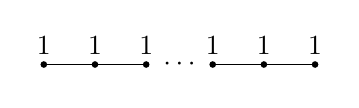
\begin{tikzpicture}[x=.65cm,y=.45cm,baseline]
\draw (0,0)--(2,0) (3.3,0)--(5.3,0);\node at (2.65,0){$\cdots$};
\foreach \x in {0,1,2,3.3,4.3,5.3}{\fill (\x,0) circle (1.2pt);\node[above] at (\x,0){$1$};}
\end{tikzpicture}&A_n,\quad n\geq1.\\[1.2em]
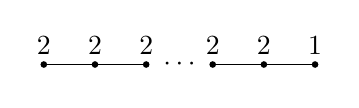
\begin{tikzpicture}[x=.65cm,y=.45cm,baseline]
\draw (0,0)--(2,0) (3.3,0)--(5.3,0);\node at (2.65,0){$\cdots$};
\foreach \x in {0,1,2,3.3,4.3}{\fill (\x,0) circle (1.2pt);\node[above] at (\x,0){$2$};}
\fill (5.3,0) circle (1.2pt);\node[above] at (5.3,0){$1$};
\end{tikzpicture}&B_n,\quad n\geq2.\\[1.2em]
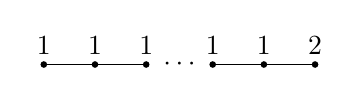
\begin{tikzpicture}[x=.65cm,y=.45cm,baseline]
\draw (0,0)--(2,0) (3.3,0)--(5.3,0);\node at (2.65,0){$\cdots$};
\foreach \x in {0,1,2,3.3,4.3}{\fill (\x,0) circle (1.2pt);\node[above] at (\x,0){$1$};}
\fill (5.3,0) circle (1.2pt);\node[above] at (5.3,0){$2$};
\end{tikzpicture}&C_n,\quad n\geq3.\\[1.5em]
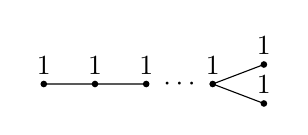
\begin{tikzpicture}[x=.65cm,y=.45cm,baseline]
\draw (0,0)--(2,0) (3.3,0)--(4.3,.55) (3.3,0)--(4.3,-.55);\node at (2.65,0){$\cdots$};
\foreach \x/\y in {0/0,1/0,2/0,3.3/0,4.3/.55,4.3/-.55}{\fill (\x,\y) circle (1.2pt);\node[above] at (\x,\y){$1$};}
\end{tikzpicture}&D_n,\quad n\geq4.\\[2em]
\begin{tikzpicture}[x=.65cm,y=.45cm,baseline]
\draw (1,0)--(2,0) (3.3,0)--(5.3,0) (3.3,0)--(3.3,-1.1);\node at (2.65,0){$\cdots$};
\foreach \x in {1,2,3.3,4.3,5.3}{\fill (\x,0) circle (1.2pt);\node[above] at (\x,0){$1$};}
\fill (3.3,-1.1) circle (1.2pt);\node[right] at (3.3,-1.1){$1$};
\end{tikzpicture}&E_n,\quad n=6,7,8.\\[1.5em]
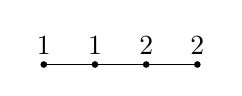
\begin{tikzpicture}[x=.65cm,y=.45cm,baseline]
\draw (2.3,0)--(5.3,0);
\foreach \x/\v in {2.3/1,3.3/1,4.3/2,5.3/2}{\fill (\x,0) circle (1.2pt);\node[above] at (\x,0){$\v$};}
\end{tikzpicture}&F_4.\\[1.2em]
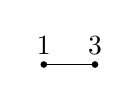
\begin{tikzpicture}[x=.65cm,y=.45cm,baseline]
\draw (4.3,0)--(5.3,0);
\foreach \x/\v in {4.3/1,5.3/3}{\fill (\x,0) circle (1.2pt);\node[above] at (\x,0){$\v$};}
\end{tikzpicture}&G_2.
\end{array}
\]
由 7.4.5 立即得到相应的群 $E_\Delta(\mathscr R)$：
\[\begin{aligned}
E_\Delta(\mathscr R)&=\{e\}&&\text{对 }A_1,B_n,C_n,E_7,E_8,F_4,G_2,\\
E_\Delta(\mathscr R)&=\mathbb Z/2\mathbb Z&&\text{对 }A_n\ (n\geq2),D_n\ (n\geq5),E_6,\\
E_\Delta(\mathscr R)&=\mathfrak S_3&&\text{对 }D_4.
\end{aligned}\]
\textbf{7.5. 关于 $p$-\Term{morphism}{态射}的补充。}
设 $f:\mathscr R\to\mathscr R'$ 为\Term{p-morphism}{$p$-态射}（参见 6.8）。从定义显然可见，与 $f$ 关联的\Term{bijection}{双射} $u:R\xrightarrow\sim R'$ 使 $R$ 与 $R'$ 的\Term{simple-root-system}{单根系}、\Term{positive-root-system}{正根系}、\Term{irreducible-root-datum}{不可约分支}等相互对应。为简便起见，假设 $R$ 与 $R'$ 都\Term{irreducible-root-datum}{不可约}。
\begin{SGAresult}{引理}{7.5.1}
若 $R$ 与 $R'$ 都\Term{irreducible-root-datum}{不可约}，则存在 $k\in\mathbb Q$，使对每个 $\alpha\in R$ 有
\[k\operatorname{long}(u(\alpha))=q(\alpha)^2\operatorname{long}(\alpha).\]
\end{SGAresult}
\SourcePage{107}
\begin{proof}
事实上，有 $\operatorname{long}(\alpha)(\alpha^*,\beta)=\operatorname{long}(\beta)(\beta^*,\alpha)$，同样有
\[\operatorname{long}(u(\alpha))(u(\alpha)^*,u(\beta))
=\operatorname{long}(u(\beta))(u(\beta)^*,u(\alpha)).\]
于是立即得出，对不\Term{orthogonality}{正交}的 $\alpha,\beta$，有
\[\frac{q(\alpha)^2\operatorname{long}(\alpha)}{\operatorname{long}(u(\alpha))}
=\frac{q(\beta)^2\operatorname{long}(\beta)}{\operatorname{long}(u(\beta))},\]
再由 7.1.3 (iv) 得到结论。
\end{proof}
\textbf{注记 7.5.2。}由 7.2.2 和 6.8.4 可知，$q(\alpha)$ 只依赖于 $\operatorname{long}(\alpha)$。于是容易看出，若 $q(\alpha)$ 不是常数，则 $q(\alpha)\operatorname{long}(\alpha)$ 是常数，从而此时 $p=2$ 或 $3$。观察上一节的图可见有四种可能（用同一字母表示一个\Term{dynkin-diagram}{Dynkin 图}及相应的\Term{reduced}{约化}\Term{simply-connected-root-datum}{单连通根数据}）：
\[\begin{aligned}
p=2,&\quad B_n\xrightarrow{f_1}C_n,\qquad C_n\xrightarrow{f_2}B_n\quad(\text{其中 }C_2=B_2),\\
p=2,&\quad F_4\xrightarrow g F_4,\\
p=3,&\quad G_2\xrightarrow h G_2.
\end{aligned}\]
读者会注意到，$f_1\circ f_2$、$f_2\circ f_1$、$g\circ g$ 和 $h\circ h$ 都是 6.8.6 所述\Term{form}{形式}的\Term{p-morphism}{$p$-态射}。

\textbf{7.5.3。}由上述描述立即可见，若 $\mathscr R,\mathscr R'$ 是两个\Term{semisimple-rank}{半单秩}至多为 $2$ 的\Term{reduced-root-datum}{约化根数据}，且存在从 $\mathscr R'$ 到 $\mathscr R$ 的\Term{p-morphism}{$p$-态射}，则 $\mathscr R$ 与 $\mathscr R'$ 具有相同的类型。更确切地说，有下表。

\textit{记号：}设 $f:\mathscr R'\to\mathscr R$ 是\Term{p-morphism}{$p$-态射}。以 $q$（分别地，$q_1$）表示 $p$ 的任意正幂。对秩为 $2$ 的\Term{root-system}{根系}，采用第 4 节的记号（以 $\alpha,\beta$ 表示\Term{simple-root}{单根}，使 $\ell(\alpha)\leq\ell(\beta)$）。
\[
\begin{array}{|c|c|c|c|}\hline
\text{类型}&p&f\text{ 的值}&{}^tf\text{ 的值}\\\hline
\text{平凡}&\text{任意}&-&-\\\hline
A_1&\text{任意}&f(\alpha')=q\alpha&{}^tf(\alpha^*)=q\alpha'^*\\\hline
A_1\times A_1&\text{任意}&f(\alpha')=q\alpha&{}^tf(\alpha^*)=q\alpha'^*\\
&&f(\beta')=q_1\beta&{}^tf(\beta^*)=q_1\beta'^*\\\hline
A_2,B_2,G_2&\text{任意}&f(\alpha')=q\alpha&{}^tf(\alpha^*)=q\alpha'^*\\
&&f(\beta')=q\beta&{}^tf(\beta^*)=q\beta'^*\\\hline
B_2&p=2&f(\alpha')=q\beta&{}^tf(\alpha^*)=2q\beta'^*\\
&&f(\beta')=2q\alpha&{}^tf(\beta^*)=q\alpha'^*\\\hline
G_2&p=3&f(\alpha')=q\beta&{}^tf(\alpha^*)=3q\beta'^*\\
&&f(\beta')=3q\alpha&{}^tf(\beta^*)=q\alpha'^*\\\hline
\end{array}
\]
\SourcePage{108}
\textbf{参考文献}
\begin{description}
\item[{[BLie]}] N. Bourbaki，《群与 \Term{lie-algebra}{Lie 代数}》（\textit{Groupes et algèbres de Lie}），第 IV--VI 章，Hermann，1968。
\item[{[De80]}] M. Demazure，\textit{A,B,C,D,E,F, etc.}，第 221--227 页，载于《曲面奇点讨论班》（\textit{Séminaire sur les singularités des surfaces}，Palaiseau，1976--1977），M. Demazure、H. C. Pinkham、B. Teissier 编，\textit{Lect. Notes Math.} 777，Springer-Verlag，1980。
\end{description}
